%!TEX root = paper_ecg_cs_codec.tex
\section{Experiments and Discussion}
\label{sec:results}
The experiments in this section have been
designed to study the compression efficiency
of the encoder and the quality of reconstruction
under different reconstruction algorithms.


\subsection{Gaussianity}

The key idea behind our entropy coding
design is to model the measurement values as
being sampled from a quantized Gaussian distribution.
\Cref{fig-cs-codec:y:hist:200} shows the histograms of measurement
values for 6 different records.
Gaussian distribution is not a very bad approximation visually.

The best compression can be achieved by using the empirical
probabilities of different values in $\by$ in an entropy model.
However, doing so would require us to transmit the empirical
probabilities as side information. This may be expensive.
We can estimate the improvement in compression overhead
by use of the quantized Gaussian approximation.
Let $\PP$ denote the empirical probability distribution
of data and let $\QQ$ denote the corresponding
quantized Gaussian distribution. Bamler in \cite{bamler2022constriction}
show empirically that the overhead of using an approximation
distribution $\QQ$ in place of $\PP$ in ANS entropy coding
is close to the KL divergence $\text{KL}(\PP || \QQ)$
which is given by
\begin{equation}
\text{KL}(\PP || \QQ) = \sum_y \PP(y) \log_2\left (\frac{\PP(y)}{\QQ(y)} \right).
\end{equation}
We computed the empirical distribution for $\by$ for each
record and measured its KL divergence with the corresponding
quantized Gaussian distribution.
It varies around $0.11 \pm 0.07$ bits across the 48 records
for an encoder configuration with $m=256,n=512,d=4$.
Thus, the overhead of using a quantized
Gaussian distribution in place of the empirical probabilities
can be estimated to be $4-18\%$.
The empirical distributions vary widely from one record to another
in the database. Hence using a single fixed empirical distribution
(e.g. the Huffman codebook preloaded into the device in
\cite{mamaghanian2011compressed})
may lead to lower compression.

\begin{figure}
\centering % <-- added
\subfloat[Record 100]{%
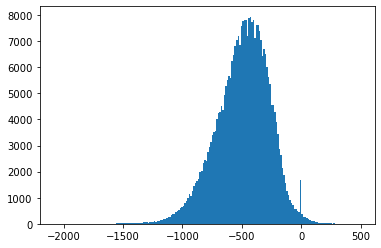
\includegraphics[width=0.3\linewidth]{images/rec_100_hist_measurements_200_bins.png}}
\hfill
\subfloat[Record 102]{%
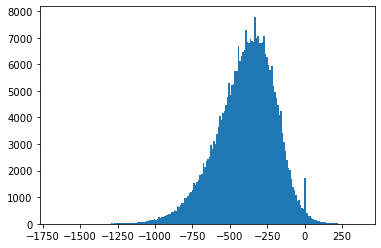
\includegraphics[width=0.3\linewidth]{images/rec_102_hist_measurements_200_bins.png}}
\hfill
\subfloat[Record 115]{%
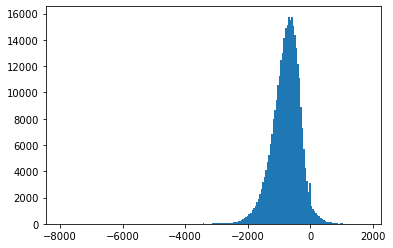
\includegraphics[width=0.3\linewidth]{images/rec_115_hist_measurements_200_bins.png}}
\\
\subfloat[Record 202]{%
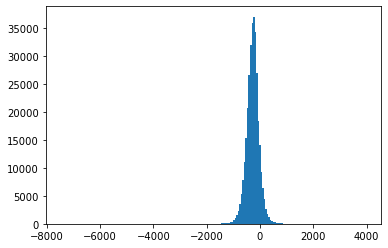
\includegraphics[width=0.3\linewidth]{images/rec_202_hist_measurements_200_bins.png}}
\hfill
\subfloat[Record 208]{%
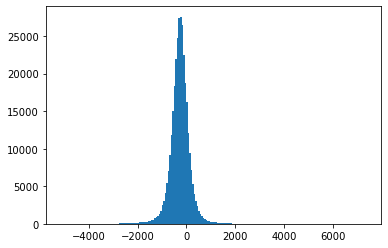
\includegraphics[width=0.3\linewidth]{images/rec_208_hist_measurements_200_bins.png}}
\hfill
\subfloat[Record 234]{%
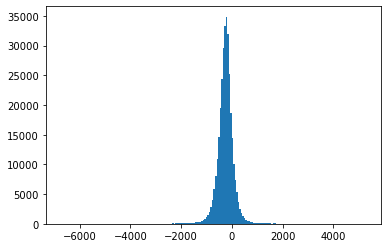
\includegraphics[width=0.3\linewidth]{images/rec_234_hist_measurements_200_bins.png}}
\caption{Histograms of measurement values with the sparse binary sensing matrix
with $m=256,n=512,d=4$ in 200 bins}
\label{fig-cs-codec:y:hist:200}
\end{figure}


\subsection{Quantization Parameter}

\begin{figure*}
\centering
\subfloat[$q$ vs $\prd$]{%
\includegraphics[width=0.32\linewidth]{images/rec_100_q_vs_prd_at_mr.pdf}}
\hfill
\subfloat[$q$ vs $\pss$]{%
\includegraphics[width=0.32\linewidth]{images/rec_100_q_vs_pss_at_mr.pdf}}
\hfill
\subfloat[$\pms$ vs $\pss$]{%
\includegraphics[width=0.32\linewidth]{images/rec_100_pms_vs_pss_at_q.pdf}}
\hfill
\caption{Variation of compression statistics vs quantization parameter
at different measurement ratios $\frac{m}{n}$
for record 100}
\label{fig-cs-codec-100-q-mr-stats}
\end{figure*}


The quantization step is a key contributor to compression
savings. This can be studied better under the fixed
quantization mode. In the first experiment, we compress
the data from record 100 at different values of
the quantization parameter $q$ and PMS.
The results are shown in \cref{fig-cs-codec-100-q-mr-stats}.
The number of measurements ($m$) has been chosen to vary from
$20\%$ to $60\%$ of the window size ($n$).
$q$ varies from $0$ to $7$.
(a) shows that reconstruction quality doesn't
change much from $q=0$ till $q=4$ after which it starts degrading.
As expected, the PRD degrades as $m$ is reduced.
(b) shows that PSS (percentage space saving) increases linearly
with $q$. As $q$ increases, the size of the alphabet for
entropy coding reduces and this leads to increased space savings.
(c) shows the variation of PSS with PMS at different values of $q$.
PSS increases linearly with PMS. Also, PSS is much higher
than PMS at higher quantization levels.

Increasing quantization linearly increases the PSS.
Since up to $q=4$, there is no noticeable
impact on PRD, as seen in panel (a), it is safe
to enjoy these savings in bit rate. 
At $40\%$ PMS, one can attain up to $69.3\%$ PSS without
losing any reconstruction quality.

\Cref{fig:100:q:0-7} shows the impact of the
quantization step on the reconstruction quality
for a small segment of record 100.
The first panel shows the original (digital) signal.
The remaining panels show the reconstruction at different $q$ values
using the BSBL-BO algorithm.
The reconstruction visual quality is excellent
up to $q=5$ (PRD below 7\%), good at $q=6$ (PRD at 9\%)
and clinically unacceptable at $q=7$
(with PRD more than 15\%).
One can see significant waveform distortions at $q=7$.
Also, note how the quality score keeps increasing till
$q=4$ and starts decreasing after that with a massive
drop at $q=7$.

\begin{figure}
\centering 
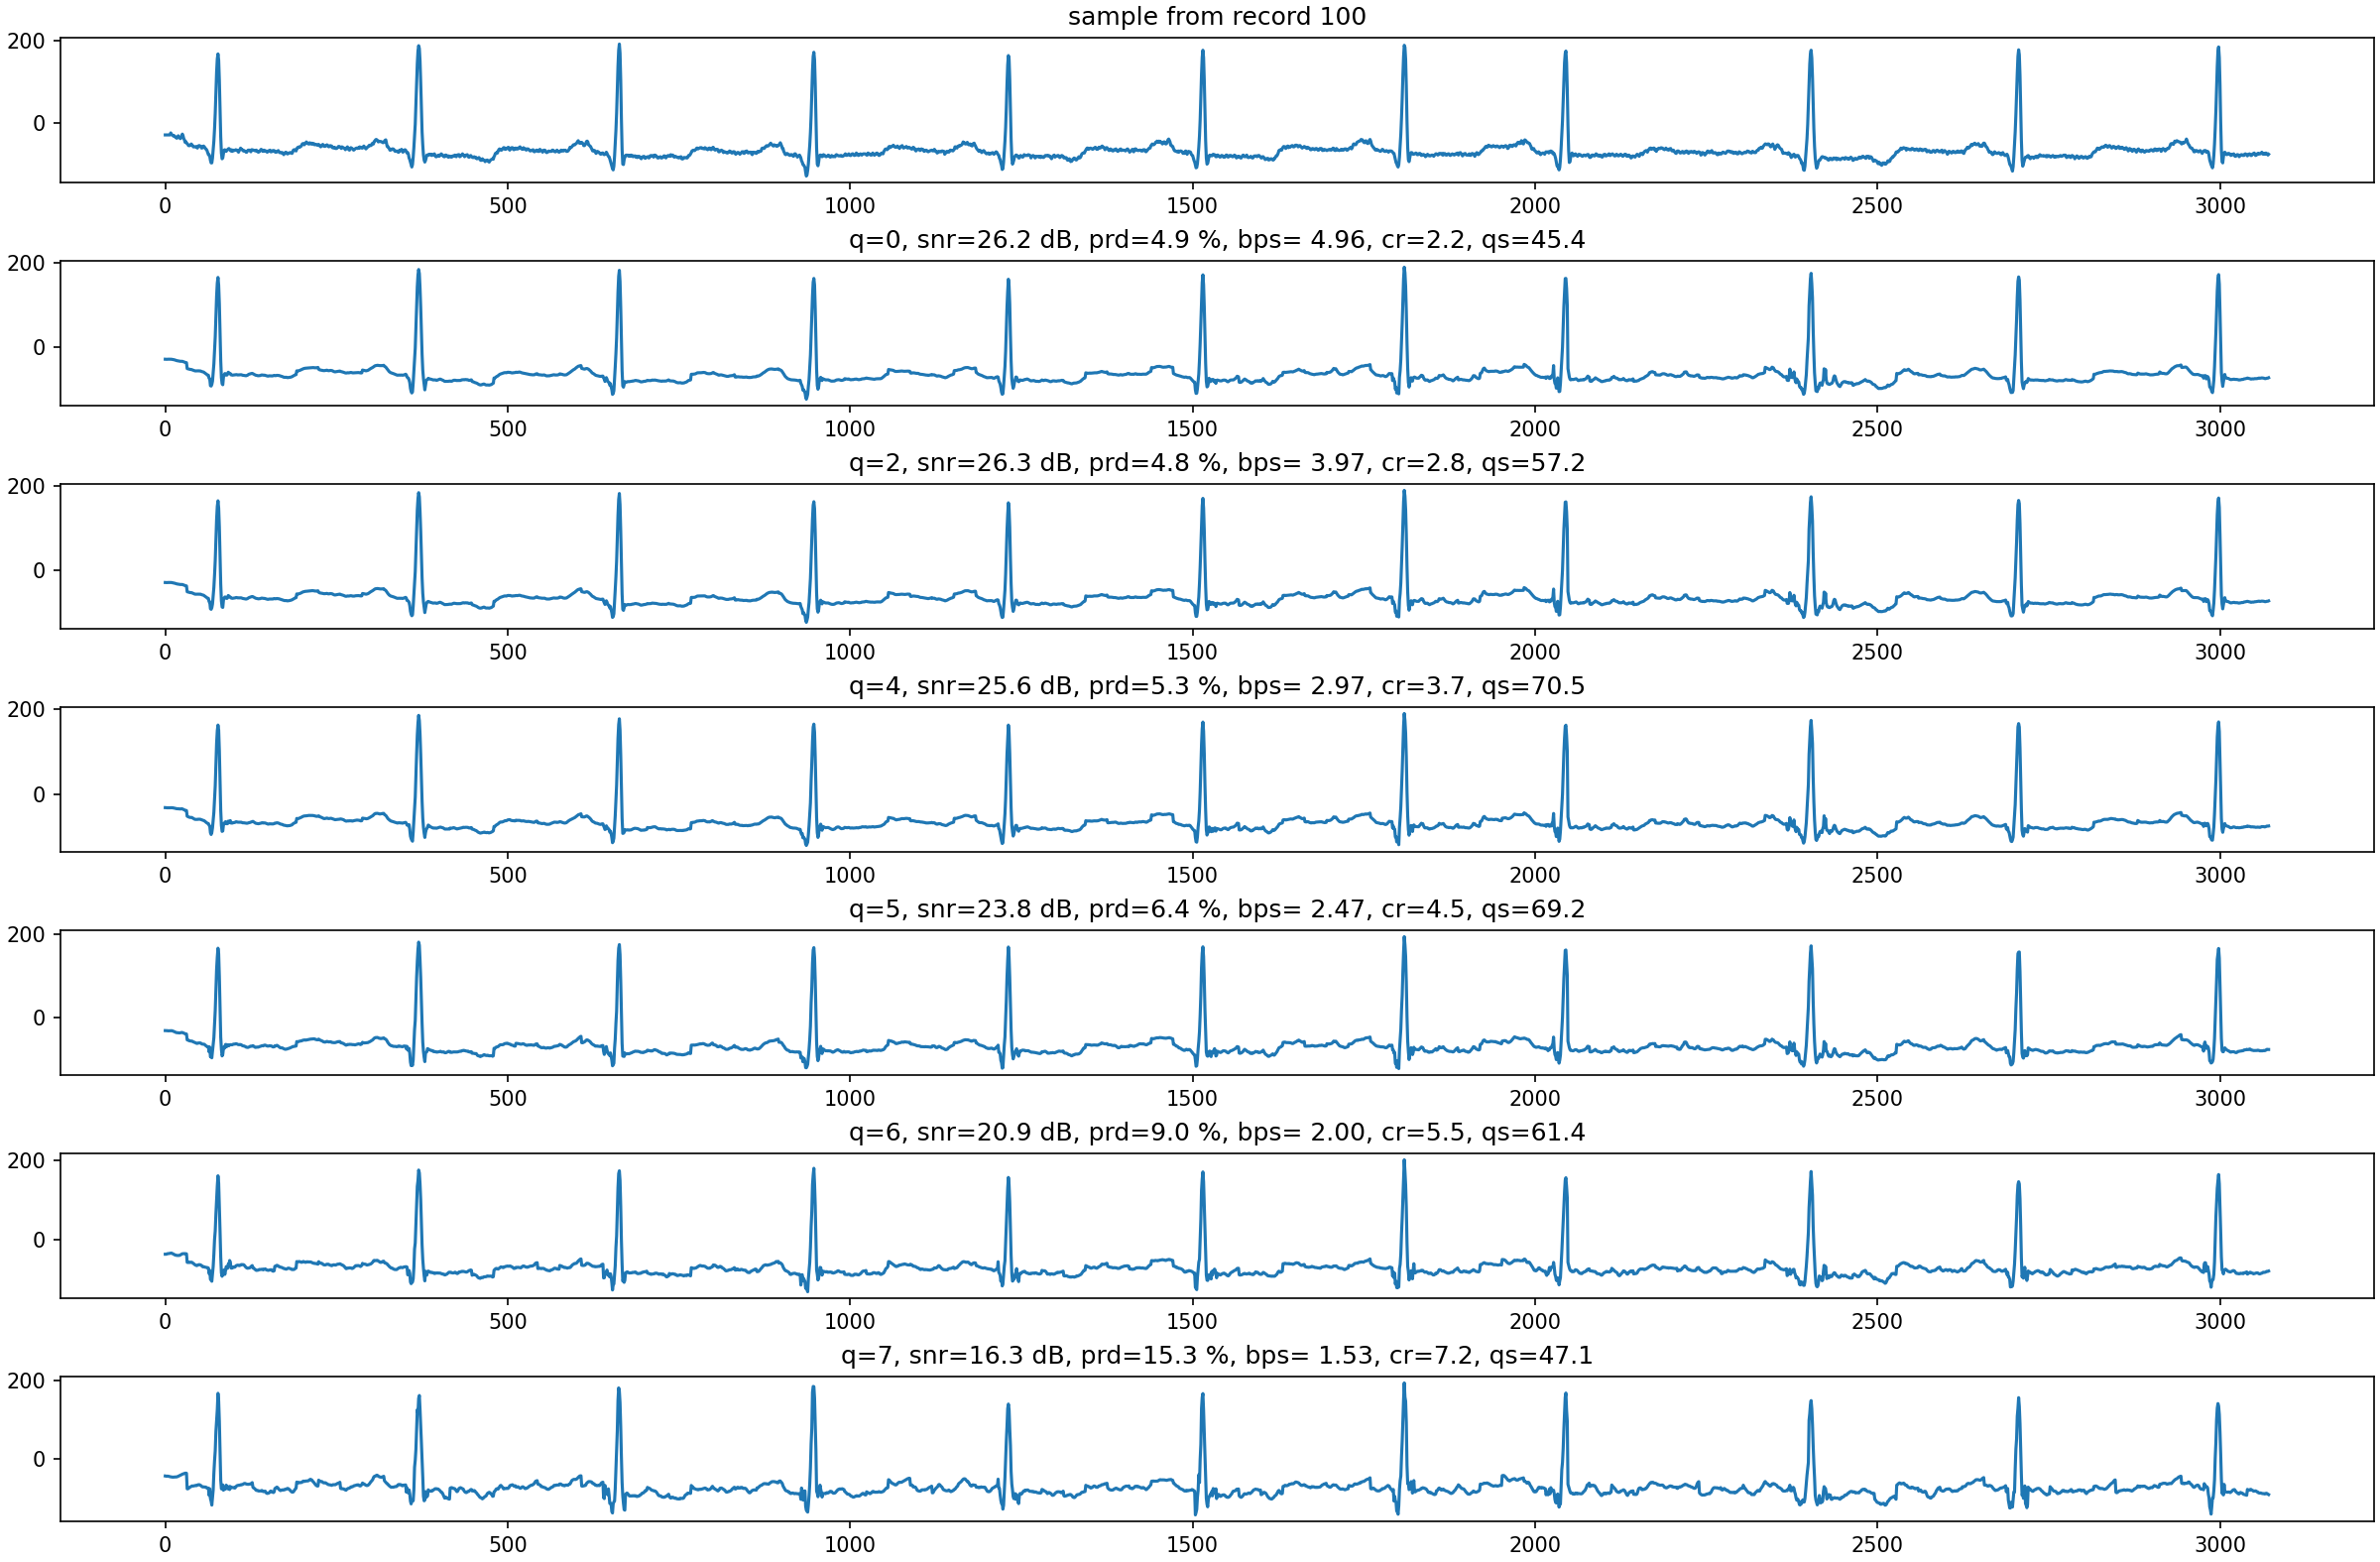
\includegraphics[width=0.95\linewidth]
{images/rec_100_q_cr_prd_qs.png}
\caption{Reconstruction of a small segment of record 100
for different values of $q=0,2,4,5,6,7$ with $m=256,n=512,d=4$
under non-adaptive quantization.
The block size for the BSBL-BO decoder is $32$.}
\label{fig:100:q:0-7}
\end{figure}
In the remaining experiments, we will be using adaptive
quantization.

We note that Mamaghanian et al. \cite{mamaghanian2011compressed}
have used an inter-packet redundancy removal step before
Huffman coding. They suggest that measurements of consecutive
windows are correlated due to the periodic nature of the ECG signal.
However, we suspect that this was happening due to the use of
unsigned digital values with a large DC component in their design.
Since we removed the baseline from the signal before compression,
we didn't notice any significant inter-packet redundancy.
Hence, we haven't included any redundancy removal block in our encoder.

\subsection{Space Savings}

In this experiment, we report the variation of
the percentage space savings ($\pss$)
with the percentage measurement savings ($\pms$)
under different encoder configurations.
We chose the window size $n=512$.
PMS varies from $20\%$ to $80\%$.
Correspondingly $m$ varies from $410$ down to $77$.
For each choice of $m$ and $n$, we constructed
binary sensing matrices $\Phi$
for two different values of $d$ at $d=4$ and $d=12$.
All 48 records were encoded and $\pss$ was measured
separately for each of them.
\Cref{fig-res-pms-pss-errorbar} shows the variation
of mean $\pss$ (over records) with $\pms$ along with
error bars for standard deviation across records
at each $\pms$.
We note that $d=12$ gives slightly better compression.
However, the difference is not significant and it decreases
as PMS increases. The small error bars indicate that the
compression ratio doesn't vary much from record to record.
At low PMS, we can see that the compression scheme can
give additional savings of up to 25\%. The trend line
is linear and savings reduce linearly to 5\% at 85\% PMS.

\begin{figure}
\centering
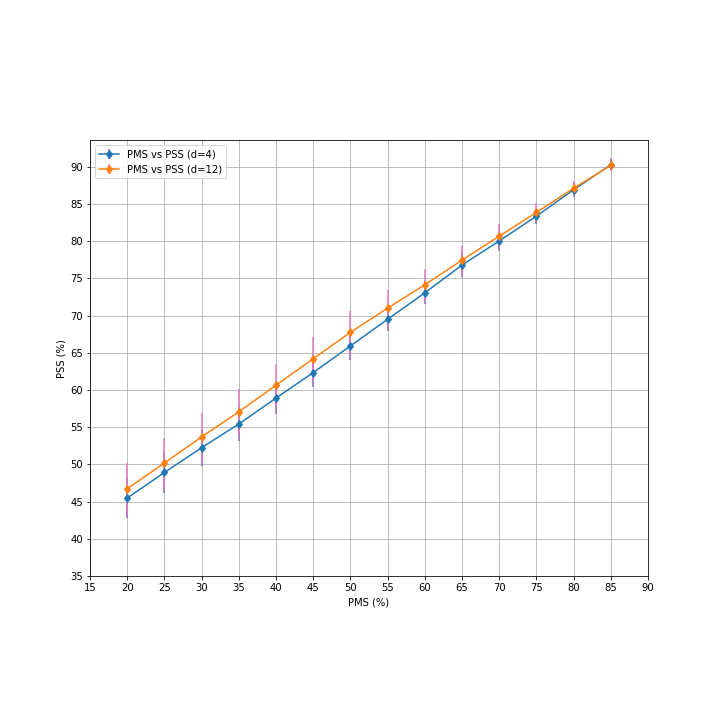
\includegraphics[width=0.95\linewidth]{images/bsbl/pms-vs-pss-errorbar.png}
\caption{Error bars for variation of mean $\pss$
with $\pms$ for 48 records at $d=4$ and $d=12$.}
\label{fig-res-pms-pss-errorbar}
\end{figure}

\Cref{fig-res-pms-pss-boxplot-d4} shows more detailed box plots
of variation of PMS across the 48 records at different PMS values.

\begin{figure}
\centering
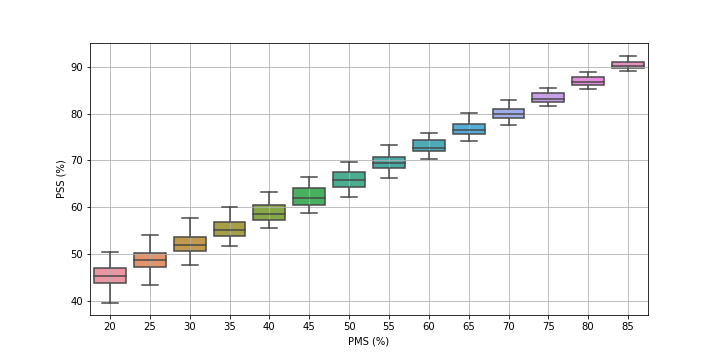
\includegraphics[width=0.95\linewidth]{images/bsbl/pms-vs-pss-boxplot-d4.png}
\caption{PMS vs PSS box plots over 48 records at $d=4$}
\label{fig-res-pms-pss-boxplot-d4}
\end{figure}
In the following, we will report results for $d=4$
configuration. Results are similar for $d=12$.

We measured the overhead of bits required to
encode the stream and frame headers. The overhead
varies from 0.07\% at PMS=20\% to about 0.4\% at PMS=80\%
on average. At higher PMS there are very few measurements
to encode. Hence overhead is higher. Increasing the frame
size will reduce the overhead. However, this will cause
delays in a real-time system since a frame cannot be decoded
till its full payload has been received. 

The bits per sample vary from
$6 \pm 0.3$ $\bps$ at PMS=20\% down to
$1 \pm 0.1$ $\bps$ at PMS=85\%.
This is significant compared to the uncompressed
rate of $11$ bits per sample.

Savings gain can be measured as the difference $\pss - \pms$.
\Cref{fig-res-pms-gain-boxplot-d4} shows the box plots of
savings gains at different PMS levels.
Savings gain varies from $25\pm3\%$ at PMS=20\% down to
$5.3 \pm 0.9\%$ at PMS=85\%. More measurements lead to
more savings via the quantization, clipping and entropy coding steps.


\begin{figure}
\centering
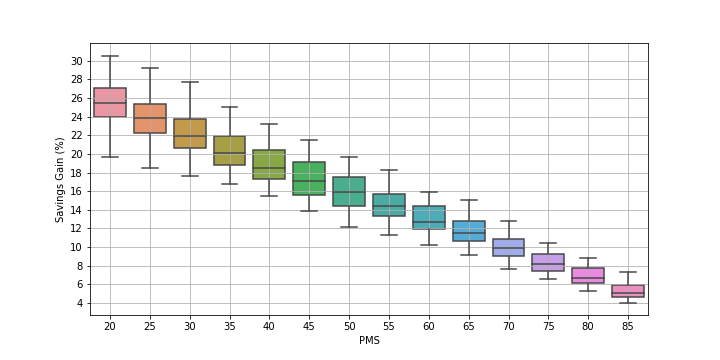
\includegraphics[width=0.95\linewidth]{images/bsbl/pms-vs-saving-gain-boxplot.png}
\caption{PMS vs Savings gain (PSS - PMS) box plots over 48 records at $d=4$}
\label{fig-res-pms-gain-boxplot-d4}
\end{figure}

Our adaptive quantization scheme is designed to
keep the noise introduced by quantization and clipping
steps to reasonable levels.
\Cref{fig-res-pms-q-snr-boxplot-d4} shows the box plots
of variation of quantization noise SNR across the 48
records at different PMS. It is clear that quantization
SNR remains limited between 35 and 40 dB.

\begin{figure}
\centering
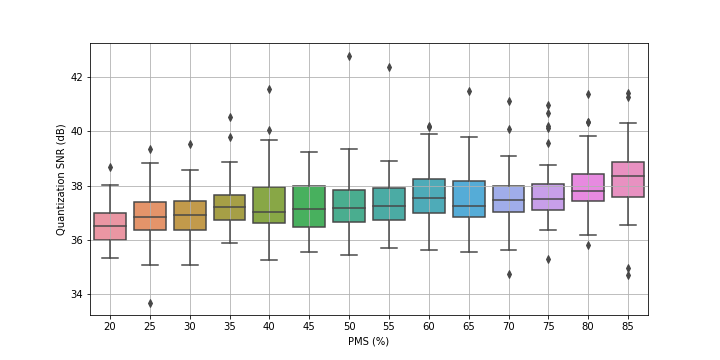
\includegraphics[width=0.95\linewidth]{images/bsbl/pms-vs-q-snr-boxplot-d4.png}
\caption{PMS vs Quantization SNR box plots over 48 records at $d=4$}
\label{fig-res-pms-q-snr-boxplot-d4}
\end{figure}

Compression is to no avail if the signal cannot be reconstructed
faithfully. The reconstruction heavily depends
on the choice of the sparse recovery algorithm.
In the following, we present our results for two different sparse
recovery approaches.

\subsection{Reconstruction with BSBL-BO}

\Cref{fig-res-bsbl-pms-prd-errorbar} shows the variation
of mean PRD with PMS for $d=4$ as well as $d=12$ when BSBL-BO
reconstruction algorithm is used in the decoder. The error
bars show the standard deviation of PRD across the 48 records.
We have drawn additional lines for 2\% and 9\% PRD that indicate
very good and good reconstruction levels. 
Surprisingly, $d=4$ gives us better PRD. 
We can see that mean PRD is below 9\% level till up to 65\% PMS.
At this PMS, we have a PSS of about 77\% (\cref{fig-res-pms-pss-errorbar}).

\begin{figure}
\centering
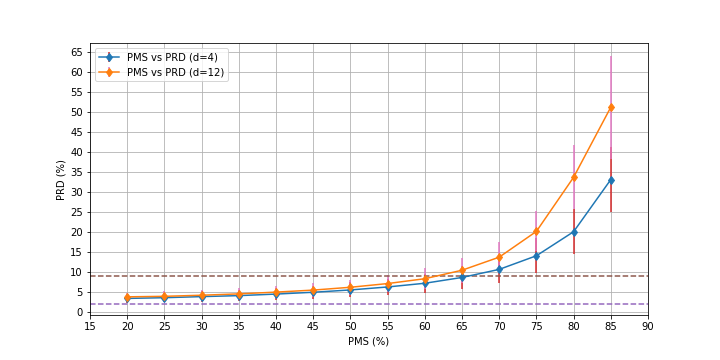
\includegraphics[width=0.95\linewidth]{images/bsbl/pms-vs-prd-errorbar.png}
\caption{Error bars for variation of PMS vs mean PRD at $d=4$ and $d=12$
for reconstruction with the BSBL-BO algorithm.}
\label{fig-res-bsbl-pms-prd-errorbar}
\end{figure}


% \begin{figure}
% \centering
% 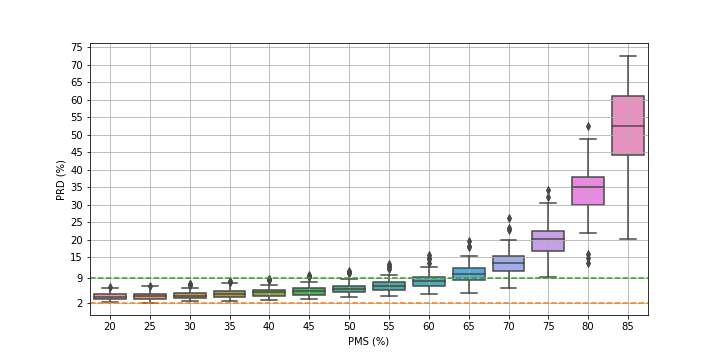
\includegraphics[width=0.95\linewidth]{images/bsbl/pms-vs-prd-boxplot-d12.png}
% \caption{PMS vs PRD box plots over 48 records at $d=12$ for reconstruction
% with the BSBL-BO algorithm.}
% \label{fig-res-bsbl-pms-prd-boxplot-d12}
% \end{figure}

\Cref{fig-res-bsbl-pms-prd-boxplot-d4} provides more detailed box plots
for the variation of PRD with PMS across the 48 records at $d=4$.
\begin{figure}[!t]
\centering
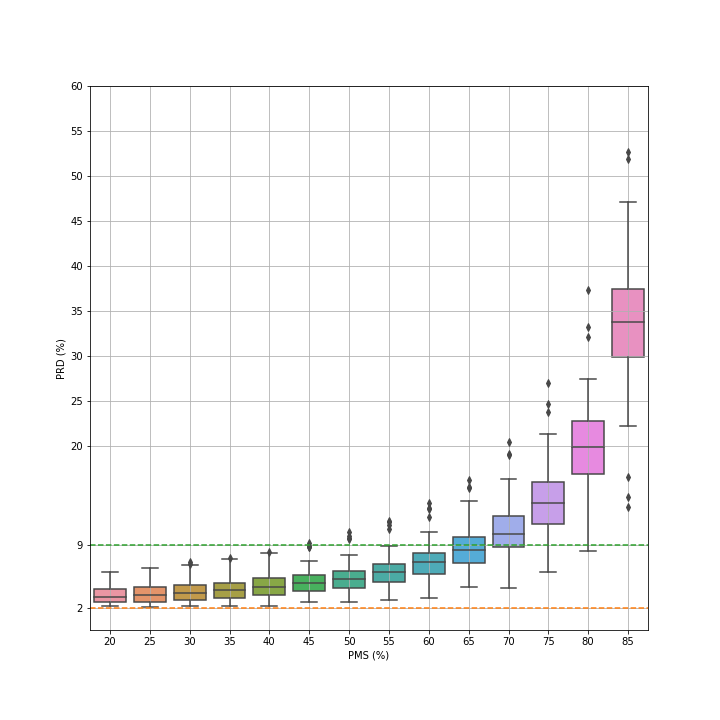
\includegraphics[width=0.95\linewidth]{images/bsbl/pms-vs-prd-boxplot-d4.png}
\caption{PMS vs PRD box plots over 48 records at $d=4$ for reconstruction
with BSBL-BO algorithm}
\label{fig-res-bsbl-pms-prd-boxplot-d4}
\end{figure}

\subsection{Reconstruction with CSNet}
For CSNet, a window size of $n=256$ was chosen following \cite{zhang2021csnet}.
We only trained and tested for a fixed binary sensing matrix with $d=4$.
\Cref{fig-res-csnet-pms-prd-boxplot} shows detailed box plots
for the variation of PRD with PMS across the 48 records.
We note that CSNet can reconstruct well up to 80\% PMS
with 7\% additional space savings (mean PSS being 87\%).
Reconstruction quality degrades far more slowly for CSNet
with mean PRD being 16.5 \% for a PMS of 90 \%
and mean PSS being 93.4\%. 

% \begin{figure}
% \centering
% 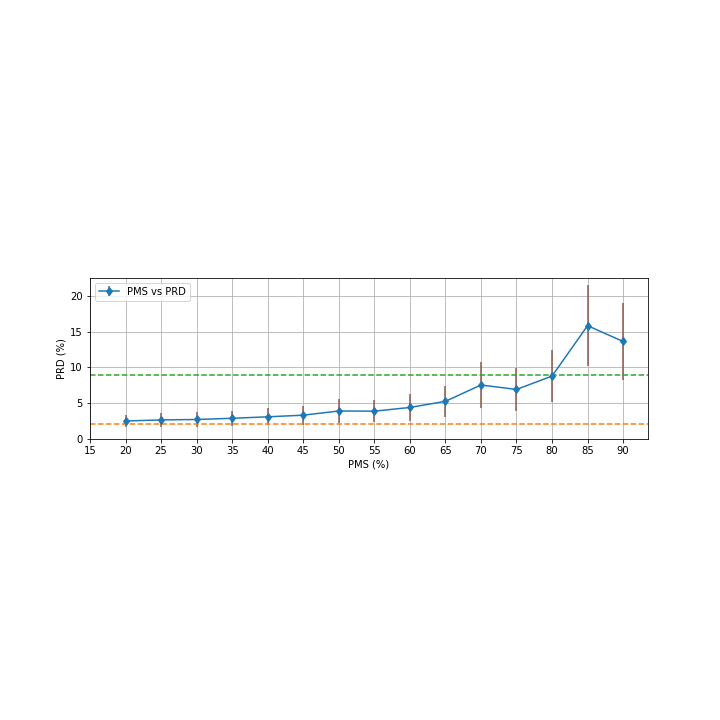
\includegraphics[width=0.95\linewidth]{images/csnet/pms-vs-prd-errorbar.png}
% \caption{Error bars for variation of mean PRD with PMS at $d=4$ for reconstruction with
% CS-NET.}
% \label{fig-res-csnet-pms-prd-errorbar}
% \end{figure}

\begin{figure}
\centering
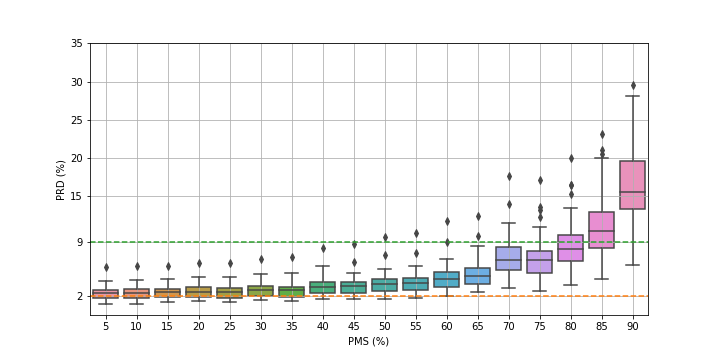
\includegraphics[width=0.95\linewidth]{images/csnet/pms-vs-prd-boxplot.png}
\caption{PMS vs PRD box plots over 48 records at $d=4$ for reconstruction
with CS-NET}
\label{fig-res-csnet-pms-prd-boxplot}
\end{figure}


\subsection{Comparison}
Zhang et al. \cite{zhang2021csnet} have reported
optimal PMS values for different methods (BP, OMP, BSBL-BO, CSNet, etc.)
for PRD=9\% for a subset of test records for $n=256$.
In their setup, $\Phi$ is RIP satisfying matrix which is different
from the binary sensing matrix used in our setup.
For BSBL-BO reconstruction,
we report the needed PMS as well as the corresponding PSS
for these records for a $\prd \leq 9 \%$.
in \cref{tbl-bsbl-optimal-pss-prd}.
While our codec requires slightly more measurements (lower PMS)
due to the sparsity of the sensing matrix, it consistently
outperforms in compression due to additional space
savings from quantization and entropy coding.
Our PSS is better by $6.5 \pm 3\%$. 

\begin{table}[ht]
\centering
\caption{Required PMS and corresponding PSS for BSBL-BO for
a target PRD $\leq 9\%$}
\begin{tabular}{rrrrr}
\toprule
 Record &  Ref PMS &  Our PMS &  PSS &  PRD \\
\midrule
100 &         71 &   66 & 78.0 &  8.8 \\
101 &         71 &   66 & 77.2 &  8.9 \\
102 &         70 &   61 & 75.8 &  8.7 \\
107 &         74 &   65 & 75.2 &  8.9 \\
109 &         75 &   70 & 78.8 &  8.7 \\
111 &         69 &   63 & 74.5 &  8.6 \\
115 &         68 &   67 & 78.4 &  8.7 \\
117 &         74 &   73 & 83.9 &  7.2 \\
118 &         76 &   70 & 81.3 &  8.2 \\
119 &         71 &   70 & 81.1 &  7.7 \\
\bottomrule
\end{tabular}
\label{tbl-bsbl-optimal-pss-prd}
\end{table}


Mamaghanian et al. \cite{mamaghanian2011compressed}
report their best result for CS for record 107
for which they report that "good" ($\prd \leq 9\%$)
signal recovery can be achieved up to a PSS of 74\%.
For our codec with BSBL-BO reconstruction, good
recovery was achieved up to a PSS of 75 \%.
